% predict_correct.tex

\begin{frame}
  \onslide<1->{\frametitle{What kind of problems are we trying to solve?} }
\begin{itemize}
  \onslide<2->{\item To estimate some quantity or quantities associated with a noisy dynamic process using 
imperfect, noisy measurements   }
\begin{itemize}
  \onslide<3->{\item May be a vector quantity: the \textbf{state} of the system or process  }
  \onslide<4->{\item Dynamic process is only modeled; not known perfectly  }
  \onslide<5->{\item We never really know the true state at any given time -- that's why weneed an estimator! }
\end{itemize}
  \onslide<6->{\item Measurements may be from multiple sensors simultaneously and/or sequentially} 

\end{itemize}
\end{frame}


\begin{frame}

  \onslide<1->{\frametitle{Recursive Predictor-Corrector Algorithm
}}
\begin{itemize}
 
  \onslide<2->{\item Goal:  Find a method to combine several measurements and produce 
the best estimate of some quantity of interest (the state of some system)}
  \onslide<3->{\item Measurements don't always happen at once.  Usually sequential.}
\begin{itemize}
  \onslide<4->{\item Hence we need an algorithm.}
  \onslide<5->{\item Preferably a recursive algorithm whereby we update (correct) our last estimate with each
new piece of measurement data }
\end{itemize}
  \onslide<6->{\item But the system whose state we want to estimate is often dynamic, i.e., changing 
with time.  So we need to take that into account (prediction).}
  \onslide<7->{\item Bottom line:  We seek a recursive predictor-corrector algorithm.}
\end{itemize}
\end{frame}



\begin{frame}
\onslide<1->{\frametitle{
Recursive Predictor-Corrector Algorithm
}}
\begin{itemize}
 
  \onslide<2->{\item Prediction:
 }
\begin{itemize}
 
  \onslide<3->{\item Kalman filter \textit{\textbf{extrapolates}} the solution from the previous 
iteration to
 the present time
}
  \onslide<4->{\item This is how we take system dynamics into account!} 
\end{itemize}
 

  \onslide<5->{\item Correction:
 }
\begin{itemize}
 
  \onslide<6->{\item Kalman filter uses measurement information to 
\textit{\textbf{update}}
 or \textit{\textbf{correct}} the prediction}
 
\end{itemize}
 
  \onslide<7->{\item And the cycle recursively begins anew!
}
\end{itemize}
\end{frame}


\begin{frame}

\frametitle{Recursive Predictor-Corrector Algorithm (Discrete System)
}


\begin{figure}
   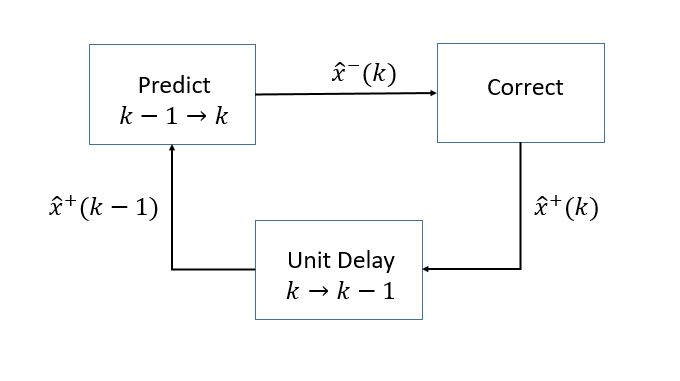
\includegraphics[width=0.75\textwidth]{day1_seg1_heuristic/pred_correct.jpg}
\end{figure}
\end{frame}


\begin{frame}
  \onslide<1->{
\frametitle{Recursive Predictor-Corrector Algorithm
} }
\begin{itemize}
 
  \onslide<2->{\item Algorithm
  }
\begin{itemize}
 
  \onslide<3->{\item Computational procedure
 }
  \onslide<4->{\item Given initial values of some quantities, new quantities are
 computed
 }
\end{itemize}
 
  \onslide<5->{\item Recursive
 }
\begin{itemize}
 
  \onslide<6->{\item The new quantities are the same as the old quantities
 }
  \onslide<7->{\item New quantities become initial values for next cycle
 }
\end{itemize}

\end{itemize}

\end{frame}
